\chapter{Morphology}
\label{sec:morphology}

There is no generic recipe on how to predict a large-scale atomistically-resolved morphology of an organic semiconductor. The required methods are system-specific: for ultra-pure crystals, for example, density-functional methods can be used provided the crystal structure is known from experiment. For partially disordered organic semiconductors, however, system sizes much larger than a unit cell  are required. Classical molecular dynamics or Monte Carlo techniques are then the methods of choice. 

In molecular dynamics, atoms are represented by point masses which interact via empirical potentials prescribed by a force-field. Force-fields are parametrized for a limited set of compounds and their refinement is often required for new molecules. In particular, special attention shall be paid to torsion potentials between successive repeat units of conjugated polymers or between functional groups and the $\pi$-conjugated system. First-principles methods can be used to characterize the missing terms of the potential energy function. 

Self-assembling materials, such as soluble oligomers, discotic liquid crystals, block copolymers, partially crystalline polymers, etc., are the most complicated to study. The morphology of such systems often has several characteristic length scales and can be kinetically arrested in a thermodynamically non-equilibrium state. For such systems, the time- and length-scales of atomistic simulations might be insufficient to equilibrate or sample desired morphologies. In this case, systematic coarse-graining can be used to enhance sampling~\cite{ruhle_versatile_2009}. Note that the coarse-grained representation must reflect the structure of the atomistic system and allow for back-mapping to the atomistic resolution.

Here we assume that the topology and the coordinates of all atoms are known. \votcactp can read standard \gromacs topology files. Custom definitions of \slink{sec:atomistic}{atomistic topology} via \xml files are also possible.


\section{Conjugated segments and rigid fragments}
\label{sec:segments}

\begin{figure}
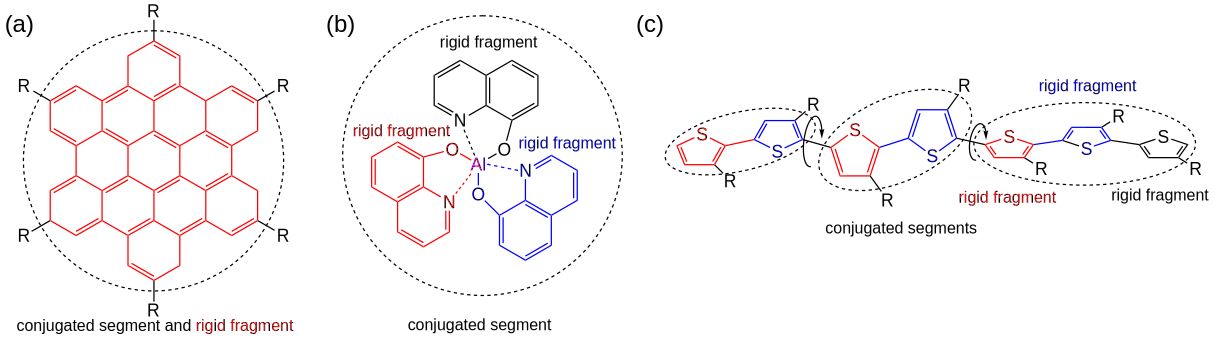
\includegraphics[width=\linewidth]{fig/fragment_segment}
\caption{The concept of conjugated segments and rigid fragments. Dashed lines indicate conjugated segments while colors denote rigid fragments. (a) Hexabenzocoronene: the $\pi$-conjugated system is both a rigid fragment and a conjugated segment. (b) \Alq: the Al atom and each ligand are rigid fragments while the whole molecule is a conjugated segment. (c) Polythiophene: each repeat unit is a rigid fragment. A conjugated segment consists of one or more rigid fragments. One molecule can have several conjugated segments.}
\label{fig:segment}
\end{figure}

With the morphology at hand, the next step is partitioning the system on hopping sites\index{hopping site}, or conjugated segments\index{conjugated segment}, and calculating charge transfer rates between them. Physically intuitive arguments can be used for the partitioning,  which reflects the localization of the wave function of a charge. For most organic semiconductors, the molecular architecture includes relatively rigid, planar $\pi$-conjugated systems, which we will refer to as rigid fragments. A conjugated segment can contain one or more of such rigid fragments, which are linked by bonded degrees of freedom. The dynamics of these degrees of freedom evolves on timescales much slower than the frequency of the internal promoting mode. In some cases, e.g. glasses, it can be `frozen' due to non-bonded interactions with the surrounding molecules.

To illustrate the concept of conjugated segments and rigid fragments, three representative molecular architectures are shown in \fig{segment}. The first one is a typical discotic liquid crystal, hexabenzocoronene. It consists of a conjugated core to which side chains are attached to aid self-assembly and solution processing. In this case the orbitals localized on side chains do not participate in charge transport and the conjugated $\pi$-system is both, a rigid fragment and a conjugated segment. 
%
In \Alq, a metal-coordinated compound, a charge carrier is delocalized over all three ligands. Hence, the whole molecule is one conjugated segment. Individual ligands are relatively rigid, while energies of the order of $k_\text{B}T$ are sufficient to reorient them with respect to each other. Thus the Al atom and the three ligands are rigid fragments.
%
In the case of a conjugated polymer, one molecule can consist of several conjugated segments, while each backbone repeat unit is a rigid fragment. Since the conjugation along the backbone can be broken due to large out-of-plane twists between two repeat units, an empirical criterion, based on the dihedral angle, can be used to partition the backbone on conjugated segments~\cite{ruhle_multiscale_2010}. However, such intuitive partitioning is, to some extent, arbitrary and shall be validated by other methods~\cite{vukmirovic_charge_2008,vukmirovic_charge_2009,mcmahon_ad_2009}. 

After partitioning, an additional step is often required to remove bond length fluctuations introduced by molecular dynamics simulations, since they are already integrated out in the derivation of the rate expression. This is achieved by substituting respective molecular fragments with  rigid, planar $\pi$-systems\index{rigid fragment} optimized using first-principles methods. Centers of mass and gyration tensors are used to align rigid fragments, though a custom definition of local axes is also possible. Such a procedure also minimizes discrepancies between the force-field and first-principles-based ground state geometries of conjugated segments, which might be important for calculations of electronic couplings, reorganization energies, and intramolecular driving forces. 

\section{Mapping file}
\label{sec:xmlmap}
The partitioning of the system on conjugated segments and rigid fragments is specified in the mapping file, \xmlcsg. Using this input, \ctpmap converts an atomistic configuration into a configuration with conjugated segments and rigid fragments and stores it in a \slink{statefile}{state file}:
%
\votcacommand{Mapping using the \gromacs topology and trajectory}{\cmdmap}
%
\ctpmap reads in the \gromacs topology from \topology, trajectory from \trajectory, definitions of conjugated segments and rigid fragments from \xmlcsg and outputs coordinates of segments and fragments to the state file, \sqlstate. After this step, dimensions of the simulation box, atom coordinates, etc, are stored in the \slink{statefile}{state file}.

\attention{\votcactp requires a wrapped \gromacs trajectory, i.~e., all molecules should be whole in the snapshot.}  

Mapping file provides three different representations of the molecule: (i) partitioning on conjugated segments and rigid fragments (mdatoms), (ii) QM-optimized geometry (qmatoms), and (iii) partitioning on electrostatic multipoles (mpoles). An example of \xmlcsg for a \dcvt molecule is shown in listing~\ref{list:map}. 

% Define new language for listings.
\lstdefinelanguage{MXML} {
   basicstyle=\ttfamily\tiny,
   sensitive=true,
   morecomment=[s][\color{gray}\rmfamily\itshape]{<!--}{-->}, 
   showstringspaces=false,
   numberstyle=\tiny,
   numberblanklines=true,
   showspaces=false,
   breaklines=true,
   showtabs=false,
   alsoletter={:},
   keywords = [1]
   { topology,molecules,molecule,name,mdname,segments,segment,fragments,fragment,mdatoms,qmatoms,mpoles,localframe,localframe_mps,orbitals,weights,weights_mps,virtual_mps,qmcoords,torbital_h, torbital_e, multipoles_n, multipoles_h, multipoles_e, map2md, U_cC_nN_h, U_nC_nN_h, U_cN_cC_h},
   keywordstyle={[1]\color{blue}},
}

\newpage
\lstinputlisting[
 language=MXML,
 label=list:map,
 caption={Examle of \xmlcsg for \dcvt. Each rigid fragment (coarse-grained bead) is defined by a list of atoms. Atom numbers, names, and residue names should correspond to those used in \gromacs topology (see the corresponing listing \ref{list:pdb} of the pdb file).}]%
{./input/dcv2t/map.xml}
\vfill

The corresponding atom numbers, names, residue numbers, and residue types of  \dcvt are shown in fig.~\ref{fig:dcv2t} and in listing~\ref{list:pdb}. \dcvt has two thiophene (THI) and two dicyanovinyl (NIT) residues, which are used to partition the molecule on four rigid fragments. Since the molecule is planar, it is represented by one conjugated segment.

\newpage
\begin{figure}[ht]
\centering
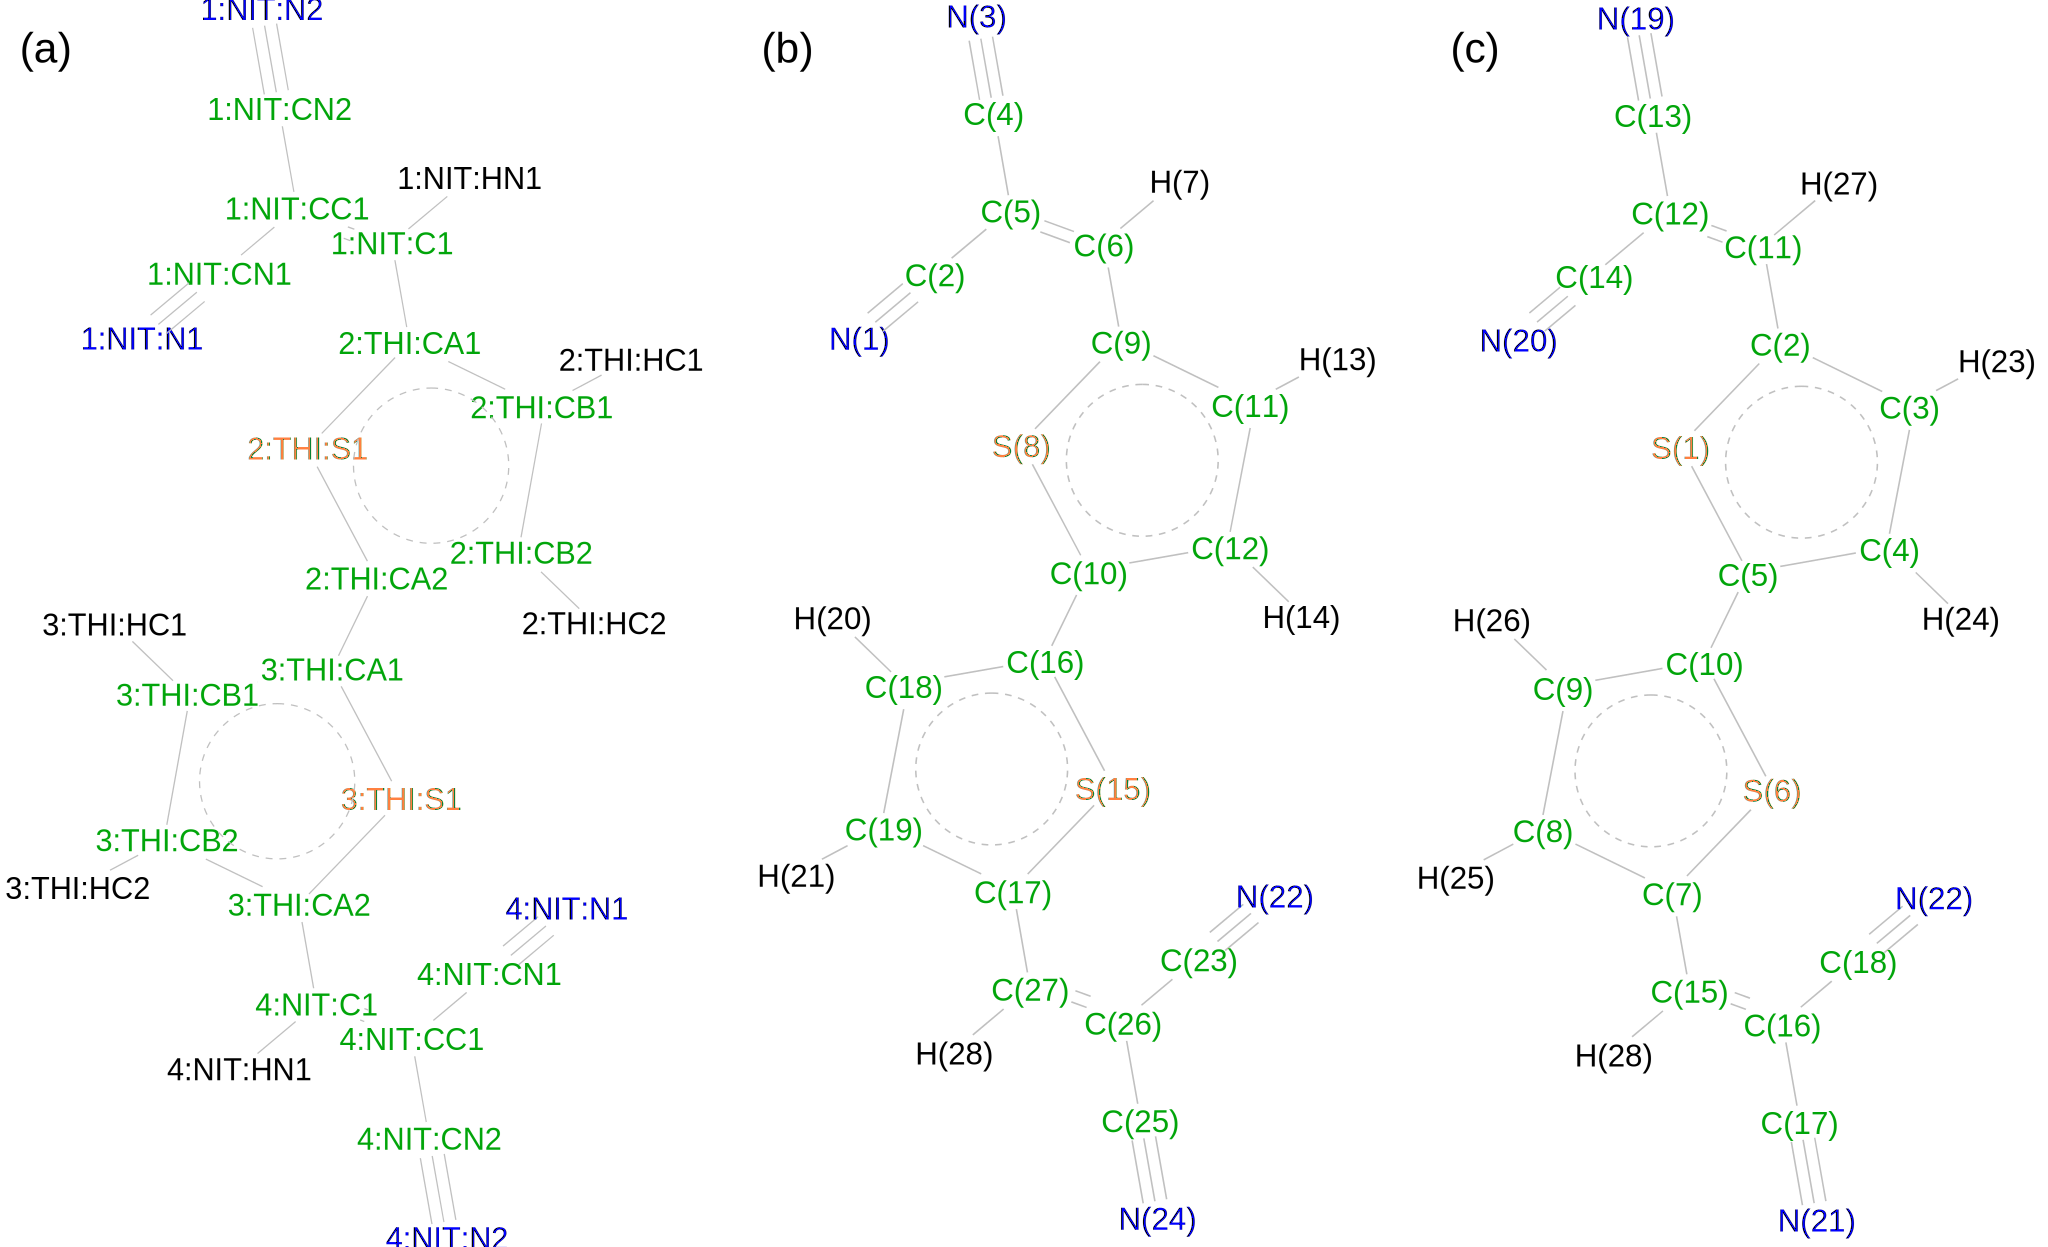
\includegraphics[width=0.8\textwidth]{./fig/dcv2t}
\caption{\small (a) \dcvt with atoms labelled according to \texttt{residue\_number:residue\_name:atom\_name}. 
There are four residues and two residue types: thiophene (THI) and dicyanovinyl (NIT). The corresponding pdb file is shown in listing~\ref{list:pdb}. Atom numbering is used to split conjugated segments on rigid fragments and to link atomistic (b) and quantum-mechanical (c) descriptions.}
\label{fig:dcv2t}
\end{figure}

\lstinputlisting[
  language=XML,
  basicstyle=\ttfamily\footnotesize,
  stringstyle=\ttfamily\footnotesize,
  showstringspaces=false,
  frame=lines,
  label=list:pdb, 
  morekeywords={HETATM,THI,NIT},
  caption={ pdb file of \dcvt.}]%
{./input/dcv2t/dcv2t.pdb}
\vfill

% PRACTICAL ADVICE
Generation of the mapping file can be semi-automatized if the atom order, residue numbering and types in the atomistic morphology reflect partitioning on rigid fragments.  This can be achieved already at the stage of preparing input files for atomistic simulations, by insuring that rigid fragments in the pdb files of all segments have   different residue types and numbers. A \dcvt pdb file, shown in listing~\ref{list:pdb}, is an example of such partitioning, where residue types (NIT and THI) and residue numbers (5-th column, from 1 to 4) uniquely define rigid fragments.

Such pdb files can be used to generate templates of \gromacs topologies, with the help of the \calc{pdb2top} tool,
\votcacommand{Creating a topol.top from a pdb file}{\small \ctptools \sql \sqlstate \exe \calc{pdb2top} }
and the mapping file, using the \calc{pdb2map} tool, 
\votcacommand{Creating a \xmlcsg from a pdb file}{\small \ctptools \sql \sqlstate \exe \calc{pdb2map} }

Both files need further refinement, but this procedure helps to avoid typos and inconsistencies between atomistic and coarse-grained morphologies.


\section{Validating the mapping}
% CHECKS
In order to visually check the mapping one can use either the \calc{tdump} \calculator or the programm \ctpdump with the calculator \calc{trajectory2pdb}.

\label{sec:ctp_dump}
\votcacommand{Writing a mapped trajectroy with \ctpdump}{\small \ctpdump \sql \sqlstate \exe \calc{trajectory2pdb} }

It reads in the state file created by \ctpmap and outputs two trajectory files corresponding to the original and rigidified atom coordinates. To check the mapping, it is useful to superimpose the three outputs (original atomistic, atomistic stored in the state file, and rigidified according to ground state geometries), e.g., with {\tt VMD}.

\label{sec:tdump}
\votcacommand{Writing a mapped trajectroy with \calc{tdump} }{\small \ctprun \sql \sqlstate \opt \xmloptions \exe \calc{tdump} }

It also reads in the state file but appends the coordinates to a pdb. file. So make sure to delete old QM.pdb and MD.pdb if you want to create a new image.


\section{Custom topologies}

\gromacs configurations and binary topologies (\texttt{topology.tpr}) can be used directly by the \ctpmap program. In this case residue and atom names should be used to specify the \slink{xmlmap}{coarse-grained topology} and \slink{xmlsegments}{conjugated segments}. 

A custom topology can also be defined using an \xml file. It is also possible to partially overwrite the information provided in, for example, \gromacs topology file. 

%We will illustrate how to create a custom topology file using \dcvt. 
